\documentclass[a4paper,15pt]{exam}
\usepackage{kotex}
\usepackage{geometry}
\usepackage{amsmath}
\usepackage{tikz}
\usetikzlibrary{positioning}
\usepackage{scalerel,amssymb}
\usepackage{calc}
\usepackage{pst-3dplot}
\geometry{margin=0.5cm}

\def \mbox {\begin{tikzpicture} \draw [draw=black](0,0) rectangle (0.3,0.3);\end{tikzpicture}}

\begin{document}

\begin{center}
  \bfseries\LARGE

  수학 \#1 \qquad 2023.01.05
  \bigskip
  \normalfont\normalsize
\end{center}


\begin{questions}
\question
    \mbox{ } 안에 들어갈 수를 쓰시오. 
    \begin{parts}
        \part 
            $ 6 \times 3 = \mbox{ } + \mbox{ } + \mbox{ } $
            \answerline
        \part 
            $ 3 \times 6 = ( 3 \times 1 ) + ( 3 \times \mbox{ } ) $
            \answerline
        \part 
            $ 3 \times 6 = 3 + ( 3 \times \mbox{ } ) $
            \answerline
        \part 
            $ 3 \times 6 = 6 + ( 3 \times \mbox{ } ) $
            \answerline
    \end{parts}

\question
    수학을 잘 하려면 수식을 잘 써내려가는 훈련이 필요합니다. 아래 수식을 그대로 똑같이 쓰세요.

    \begin{equation}
    \begin{split}
         ( 2 \times 4 ) + ( 3 \times 4 ) + ( 4 \times 3 ) & = 8 + ( 3 \times 4 ) + ( 4 \times 3 )  \\
         & = 8 + 12 + ( 4 \times 3 )  \\
         & = 8 + 12 + 12  \\
         & = 20 + 12  \\
         & = 32 
    \end{split}
    \end{equation}

    \vspace{8cm}

\question
    사과가 한 상자에 9개씩, 배가 한 상자에 6개씩 들어 있습니다. 사과 3상자와 배 4상자에 들어 있는 과일은 모두 몇 개일까요?
    \answerline

\question
    아래 곱셈표에서 곱이 20보다 큰 칸을 모두 색칠하시오. 
    \begin{center}
    \begin{tabular}{ |c|| c| c| c| c| c| c|c|}
     \hline
     $\times$ & 3 & 4 & 5 & 6 & 7 & 8 & 9 \\ 
     \hline\hline
     3 &  &   &   &   &   &   &    \\  
     \hline
     4 &  &   &   &   &   &   &    \\  
     \hline
     5 &  &   &   &   &   &   &    \\  
     \hline
    \end{tabular}
    \end{center}

    \vspace{1cm}

\question
    공을 꺼내어 공에 적힌 수만큼 점수를 얻는 놀이를 했습니다. 표를 완성하고 얻은 점수가 몇 점인지 구해보세요. 

    \begin{center}
    \begin{tabular}{ |c|| c| c| c| c|}
     \hline
     공에 적힌 수  & 3 & 4 & 5 & 6 \\
     \hline\hline
     꺼낸 횟수(번) & 2 & 3 & 1 & 0 \\
     \hline\hline
     점수(점)      & 6 &  &  & \\
     \hline
    \end{tabular}
    \end{center}

    \answerline{}


\question
    달리기 경기에서 다음과 같이 등수에 따라 점수를 얻습니다. 준기네 반에는 1등이 6명, 2등이 1명, 3등이 5명 있습니다. 준기네 반의 달리기 점수는 모두 몇 점일까요?

    \begin{center}
    \begin{tabular}{ |c|| c| c| c| }
     \hline
     등수     & 1등 & 2등 & 3등 \\
     \hline
     점수(점) & 3   & 2   & 1   \\
     \hline
    \end{tabular}
    \end{center}

    \answerline{}


\question
\mbox{ } 의 넓이를 a 라고 하자. 이때 \mbox{}\mbox{} 의 넓이는 $2 \times a $ 로 표현할 수 있다. 이때 \mbox{}\mbox{}\mbox{} 의 넓이는 $3 \times a$ 라고 할 수 있다.

\begin{parts}
    \part \mbox{}\mbox{}\mbox{}\mbox{}\mbox{}\mbox{} 의 넓이를 a 로 표현하시오. 
          \answerline
    \part 
        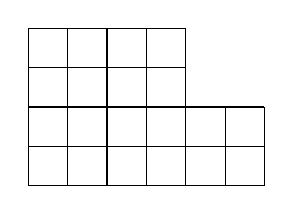
\begin{tikzpicture}
            \draw[step=0.5cm,color=black] (0,0) grid (2,2);
            \draw[step=0.5cm,color=black] (2,0) grid (3,1);
        \end{tikzpicture} 의 넓이를 $ ( \mbox{} \times 4 ) + ( \mbox{} \times 2 ) $ 로 표현했다. \mbox 에는 각각 어떤 수가 들어갈 수 있는가?
        \answerline
        \answerline

    \part
        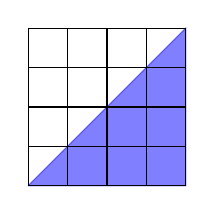
\begin{tikzpicture} 
            \draw[color=blue, fill=blue, opacity=0.5] (0,0) -- (2,2) -- (2,0) -- (0,0) ;
            \draw[step=0.5cm,color=black] (0,0) grid (2,2);
        \end{tikzpicture}

        위 그림에서 파란색 삼각형의 넓이를 a로 표현하시오.
        \answerline

    \part
        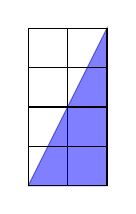
\begin{tikzpicture} 
            \draw[color=blue, fill=blue, opacity=0.5] (0,0) -- (1,2) -- (1,0) -- (0,0) ;
            \draw[step=0.5cm,color=black] (0,0) grid (1,2);
        \end{tikzpicture}

        위 그림에서 파란색 삼각형의 넓이를 a로 표현하시오.
        \answerline

\end{parts}


\question
아래와 같이 상자가 쌓여 있다고 하자. 쌓인 상자의 수는 몇개인가?

    \begin{center}
        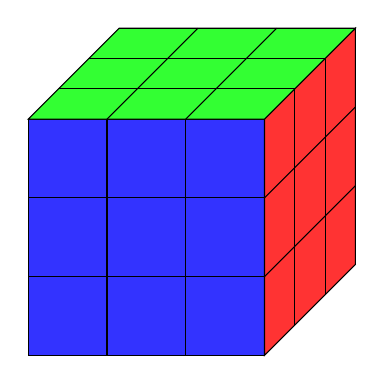
\begin{tikzpicture}
        \draw[fill=blue!80] (0,0,3)--(3,0,3)--(3,3,3)--(0,3,3)--cycle;
        \draw[fill=red!80] (3,0,0) -- (3,3,0)--(3,3,3)--(3,0,3)--cycle;
        \draw[fill=green!80] (3,3,0) -- (3,3,3)--(0,3,3)--(0,3,0)--cycle;
        \foreach \x in {1,2}
         {
        \draw(3,0,\x)--(3,3,\x); 
        \draw(3,\x,0)--(3,\x,3); 
        \draw(0,\x,3)--(3,\x,3); 
        \draw(\x,0,3)--(\x,3,3); 
        \draw(\x,3,0)--(\x,3,3); 
        \draw(0,3,\x)--(3,3,\x); 
        }
        \end{tikzpicture}
    \end{center}

\answerline

\question
빨강이는 100m를 10초에 갈 수 있다. 파랑이는 100m를 15초에 갈 수 있다. 빨강이가 빠른가? 아니면 파랑이가 빠른가?
\answerline

\question
빨강이는 100m를 10초에 갈 수 있다. 빨강이가 20초 동안 달렸을 때 몇 m까지 갈 수 있을까?
\answerline

\end{questions}
\end{document}
